% Options for packages loaded elsewhere
\PassOptionsToPackage{unicode}{hyperref}
\PassOptionsToPackage{hyphens}{url}
\PassOptionsToPackage{dvipsnames,svgnames*,x11names*}{xcolor}
%
\documentclass[
]{book}
\usepackage{lmodern}
\usepackage{amssymb,amsmath}
\usepackage{ifxetex,ifluatex}
\ifnum 0\ifxetex 1\fi\ifluatex 1\fi=0 % if pdftex
  \usepackage[T1]{fontenc}
  \usepackage[utf8]{inputenc}
  \usepackage{textcomp} % provide euro and other symbols
\else % if luatex or xetex
  \usepackage{unicode-math}
  \defaultfontfeatures{Scale=MatchLowercase}
  \defaultfontfeatures[\rmfamily]{Ligatures=TeX,Scale=1}
\fi
% Use upquote if available, for straight quotes in verbatim environments
\IfFileExists{upquote.sty}{\usepackage{upquote}}{}
\IfFileExists{microtype.sty}{% use microtype if available
  \usepackage[]{microtype}
  \UseMicrotypeSet[protrusion]{basicmath} % disable protrusion for tt fonts
}{}
\makeatletter
\@ifundefined{KOMAClassName}{% if non-KOMA class
  \IfFileExists{parskip.sty}{%
    \usepackage{parskip}
  }{% else
    \setlength{\parindent}{0pt}
    \setlength{\parskip}{6pt plus 2pt minus 1pt}}
}{% if KOMA class
  \KOMAoptions{parskip=half}}
\makeatother
\usepackage{xcolor}
\IfFileExists{xurl.sty}{\usepackage{xurl}}{} % add URL line breaks if available
\IfFileExists{bookmark.sty}{\usepackage{bookmark}}{\usepackage{hyperref}}
\hypersetup{
  pdftitle={How to be civil about political loss -- The importance of good loser messages},
  colorlinks=true,
  linkcolor=Maroon,
  filecolor=Maroon,
  citecolor=Blue,
  urlcolor=Blue,
  pdfcreator={LaTeX via pandoc}}
\urlstyle{same} % disable monospaced font for URLs
\usepackage{graphicx,grffile}
\makeatletter
\def\maxwidth{\ifdim\Gin@nat@width>\linewidth\linewidth\else\Gin@nat@width\fi}
\def\maxheight{\ifdim\Gin@nat@height>\textheight\textheight\else\Gin@nat@height\fi}
\makeatother
% Scale images if necessary, so that they will not overflow the page
% margins by default, and it is still possible to overwrite the defaults
% using explicit options in \includegraphics[width, height, ...]{}
\setkeys{Gin}{width=\maxwidth,height=\maxheight,keepaspectratio}
% Set default figure placement to htbp
\makeatletter
\def\fps@figure{htbp}
\makeatother
\setlength{\emergencystretch}{3em} % prevent overfull lines
\providecommand{\tightlist}{%
  \setlength{\itemsep}{0pt}\setlength{\parskip}{0pt}}
\setcounter{secnumdepth}{-\maxdimen} % remove section numbering
\usepackage{booktabs}
\usepackage{longtable}
\usepackage{array}
\usepackage{multirow}
\usepackage[table]{xcolor}
\usepackage{wrapfig}
\usepackage{float}
\usepackage{colortbl}
\usepackage{pdflscape}
\usepackage{tabu}
\usepackage{threeparttable}
\usepackage{threeparttablex}
\usepackage[normalem]{ulem}
\usepackage{makecell}

\title{How to be civil about political loss -- The importance of good loser
messages}
\usepackage{etoolbox}
\makeatletter
\providecommand{\subtitle}[1]{% add subtitle to \maketitle
  \apptocmd{\@title}{\par {\large #1 \par}}{}{}
}
\makeatother
\subtitle{Supporting Information}
\author{}
\date{\vspace{-2.5em}2020-08-04}

\begin{document}
\frontmatter
\maketitle

\mainmatter
\hypertarget{preface}{%
\chapter{Preface}\label{preface}}

This is the Supplementary Material for the manuscript entitled \emph{How
to be civil about political loss -- The importance of good loser
messages}.

We pre-registered Study 2 and Study 3 at aspredicted.org.

When not otherwise stated, we followed the pre-registration.

We deviated from it in the following ways:

\begin{enumerate}
\def\labelenumi{\arabic{enumi}.}
\item
  Exclusion criteria. While we registered to exclude individuals that
  raced through the survey in Study 2, we have since then learned that
  exclusion based on such a post-treatment variable can bias the
  obtained effects (Montgomery et al, 2018). Accordingly, we present the
  analysis on the full sample in the main text. The analysis using the
  reduced sample can be found in this Appendix (see section
  @ref(reduced-sample) ).
\item
  For study 2, we pre-registered a hypothesis that predicts an
  interaction between the good loser norm and the good loser message.
  Since there is little variance on the good-loser norm variable, this
  analysis is less insightful than we had anticipated. We therefore do
  not present this analysis in the main text but in the Appendix (see
  section @ref(norm-mod) ).
\item
  For study 3, we pre-registered that we would use two indicators of
  fairness perceptions. To keep the dependent variable comparable across
  studies we have later on decided to only present the analysis with the
  item: `How fair was the decision-making procedure?' for all three
  studies. The analysis using the additional item `How reasonable do you
  think the decision was?' is included in the robustness check analysis
  in the paper (Table 2).
\item
  For study 3, we missed to specify that there are two good loser
  message like in study 2 (for which we have the same expectations): A
  generic and a specific good loser message.
\item
  While we use the wording good loser prime in the pre-registration, we
  have later decided to use good loser message in the manuscript.
\end{enumerate}

\hypertarget{part-study-i}{%
\chapter{(PART) STUDY I}\label{part-study-i}}

The experiment for Study I was fielded in Sweden in the fall of 2017 and
spring of 2018 as an add-on to the fifth wave of the European Values
Survey (EVS, PI Susanne Wallman Lundåsen). EVS is based on a probability
sample of the Swedish population age 18 or older (n = 1194). Interviews
were face-to-face. The fieldwork organization was IPSOS, Sweden. For a
detailed documentation we refer to
\url{https://europeanvaluesstudy.eu/methodology-data-documentation/}.
Study 1 was one of three experiments included in a paper and pencil
leave behind. The return rate of the questionnaire was 85\% (n =1019).

\hypertarget{pre-treatment-measures-and-experimental-vignette}{%
\chapter{Pre-treatment measures and experimental
vignette}\label{pre-treatment-measures-and-experimental-vignette}}

The statistics are displayed for the respondents of interest in this
study, which is the respondents who end up with observing an unfavorable
decision outcome in the experiment.

\hypertarget{pre-treatment-measures}{%
\section{Pre-treatment measures}\label{pre-treatment-measures}}

\hypertarget{ban-on-begging---opinion}{%
\subsection{Ban on begging - opinion}\label{ban-on-begging---opinion}}

What is your opinion on a ban on begging in your municipality?

Value

N

Percent

Against ban

215

45

For ban

266

55

\hypertarget{ban-on-begging---importance}{%
\subsection{Ban on begging -
importance}\label{ban-on-begging---importance}}

How important is the issue of ban on begging to you personally?

Value

N

Percent

1 Not important at all

37

8

2

72

15

3

76

16

4

103

21

5

83

17

6

55

11

7 Very important

55

11

The mean score for the pre treatment measure ``How important is the
issue of ban on begging to you personally?'' is 4.06, and the standard
deviation is 1.76.

\hypertarget{experimental-vignette}{%
\section{Experimental vignette}\label{experimental-vignette}}

\emph{Experimental vignette.}

\begin{quote}
Imagine that your municipality is about to decide whether begging on the
streets should be banned or allowed within the municipal borders. The
decision can be made in different ways: One option is that the local
political representatives make the decision. Another option is that the
citizens of the municipality decide through a referendum. Please image
how you would react if this scenario occurred in your municipality:
After a debate in the media, the local political representatives decide
to ban begging in the municipality. \emph{Treatment text follows.}
\end{quote}

Vignette treatments and texts, Swedish vignette experiment

Treatment

Text

No prime

Imagine that your municipality is about to decide whether begging on the
streets should be banned or allowed within the municipal borders. The
decision can be made in different ways: One option is that the local
political representatives make the decision. Another option is that the
citizens of the municipality decide through a referendum. Please image
how you would react if this scenario occurred in your municipality:
After a debate in the media, the local political representatives decide
to ban begging in the municipality.

Lamenting politician

Imagine that your municipality is about to decide whether begging on the
streets should be banned or allowed within the municipal borders. The
decision can be made in different ways: One option is that the local
political representatives make the decision. Another option is that the
citizens of the municipality decide through a referendum. Please image
how you would react if this scenario occurred in your municipality:
After a debate in the media, the local political representatives decide
to ban begging in the municipality. After the decision, the leader of
one of the parties who where in favor of a ban states that they are
disappointed and that the decision was wrong.

Generic good loser prime

Imagine that your municipality is about to decide whether begging on the
streets should be banned or allowed within the municipal borders. The
decision can be made in different ways: One option is that the local
political representatives make the decision. Another option is that the
citizens of the municipality decide through a referendum. Please image
how you would react if this scenario occurred in your municipality:
After a debate in the media, the local political representatives decide
to ban begging in the municipality. After the decision, the leader of
one of the parties who where in favor of a ban states that they are
disappointed and that the decision was wrong, but that's how it is like
living in a democracy.

\hypertarget{post-treatment-measures}{%
\section{Post treatment measures}\label{post-treatment-measures}}

\hypertarget{fairness}{%
\subsection{Fairness}\label{fairness}}

What do you think about the way the decision was made?

Value

N

Percent

1 Not fair at all

74

15

2

52

11

3

77

16

4

114

24

5

54

11

6

46

10

7 Very fair

64

13

The mean score for the post treatment measure ``What do you think about
the way the decision was made?'' is 3.86, and the standard deviation is
1.91.

\hypertarget{effects-on-losers}{%
\chapter{Effects on losers}\label{effects-on-losers}}

Treatment effects on experimental subjects who find the decision outcome
to align unfavorably with their own preferences.

\hypertarget{fairness-1}{%
\section{Fairness}\label{fairness-1}}

In the manuscript, we mention that the Generic good loser message for
the respondents with an unfavorable outcome is on par with the outcome
favorability effect (difference in fairness perceptions between winners
and losers). The table below displays the outcome favorability effect,
and table `tab:1055\_post\_fairness' further below displays the
treatment effect of the Generic good loser message.

Conditional effect of outcome favorability on Generic good loser message
treatment, Study 1

Treatment value

Estimate

Std. Error

t-statistic

p value

Intercept

4.79

0.08

62.18

0

Unfavorable outcome

-0.93

0.11

-8.28

0

\hypertarget{fairness-i}{%
\subsection{Fairness I}\label{fairness-i}}

\begin{quote}
Figure 2 in the manuscript:
\end{quote}

Treatment effects on fairness perceptions of decision, Study 1

Treatment value

Estimate

Std. Error

t-statistic

p value

Not shown

3.46

0.16

22.32

0.00

Lamenting politician

0.27

0.21

1.26

0.21

Generic good loser message

0.88

0.21

4.15

0.00

\hypertarget{fairness-ii}{%
\subsection{Fairness II}\label{fairness-ii}}

\begin{quote}
Lamenting politician as reference category
\end{quote}

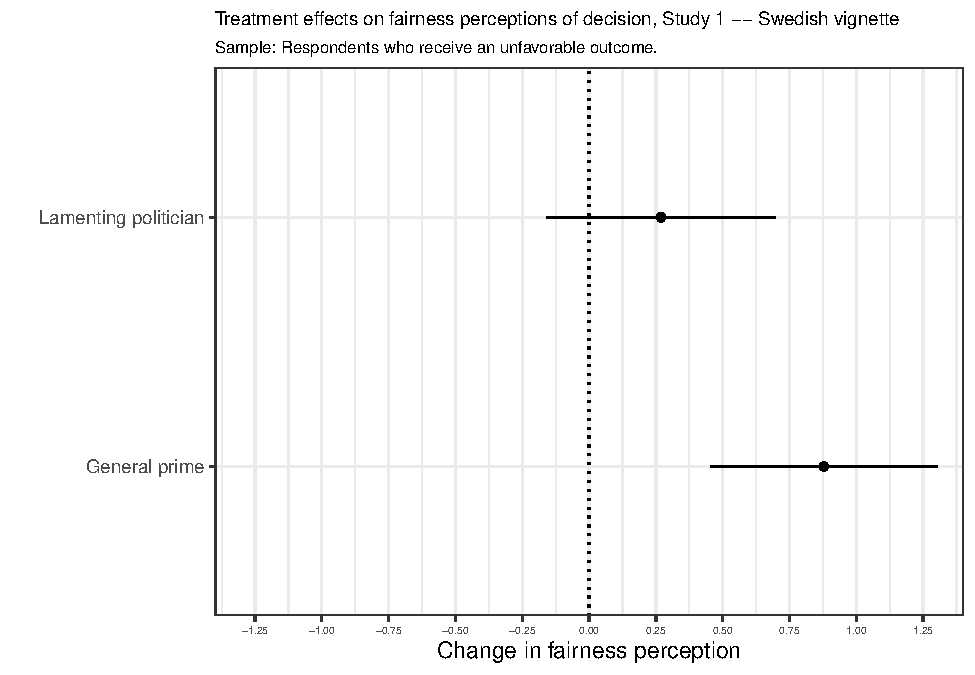
\includegraphics{Goodloser-appendix_files/figure-latex/105_post_fairness-1.pdf}

Treatment effects on fairness perceptions of decision, Study 1

Treatment value

Estimate

Std. Error

t-statistic

p value

Intercept

3.73

0.15

25.41

0.00

Not shown

-0.27

0.21

-1.26

0.21

Generic good loser message

0.61

0.21

2.96

0.00

{Note: }

Lamenting politician set as reference category.

\hypertarget{willingness-to-accept}{%
\section{Willingness to accept}\label{willingness-to-accept}}

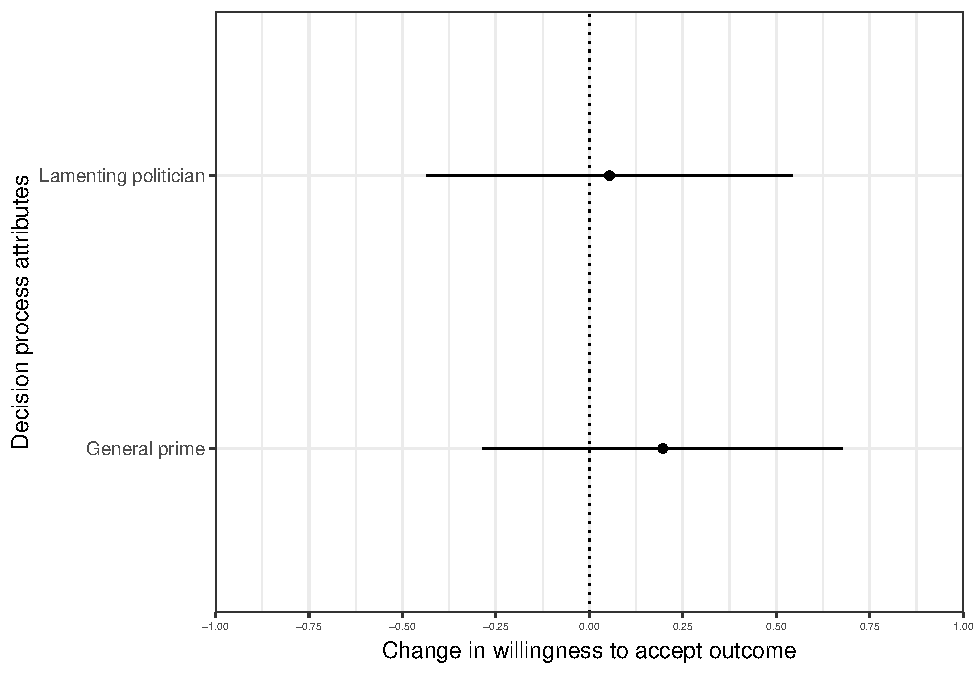
\includegraphics{Goodloser-appendix_files/figure-latex/105_post_accept-1.pdf}

Treatment effects on willingness to accept decision, Study 1

Treatment value

Estimate

Std. Error

t-statistic

p value

Not shown

4.31

0.17

24.95

0.00

Lamenting politician

-0.22

0.24

-0.93

0.35

Generic good loser message

0.13

0.24

0.57

0.57

\hypertarget{part-study-ii}{%
\chapter{(PART) STUDY II}\label{part-study-ii}}

The experiment for Study II was fielded in Norway during the spring and
fall of 2017 during the 9th and 10th waves of
\href{https://www.uib.no/medborger}{Norwegian Citizen Panel}. This is a
research-purpose internet panel with over 6000 active participants. It
is based on a probability sample of the general Norwegian population
above the age of 18 drawn from the Norwegian National Registry. The
survey is based on a online questionnaire with postal recruitment. Panel
members complete a questionnaire three times a year of 15 minutes each.
The survey panel is a core component of The Digital Social Science Core
Facilities (DIGSSCORE), and was established in 2013 as a collaboration
between several departments at the Faculty of Social Sciences at the
University of Bergen and NORCE -- Norwegian Research Centre. We refer to
the \href{Data/ncp-wave13-documentation.pdf}{documentation report} for
further details on technical aspects of the survey, panel recruitment,
response rates of the 13th wave, and representativeness. For details
about the data collected in this project and the survey panel at large,
we refer to the \href{Data/ncp-wave13-codebook.pdf}{codebook for the
Waves 1-13}.

\hypertarget{pre-treatment-vignette-post-treatment}{%
\chapter{Pre-treatment, vignette,
post-treatment}\label{pre-treatment-vignette-post-treatment}}

The statistics are displayed for the respondents of interest in this
study, which is the respondents who end up with observing an unfavorable
decision outcome in the experiment.

\hypertarget{pre-treatment-measures-1}{%
\section{Pre-treatment measures}\label{pre-treatment-measures-1}}

\hypertarget{good-loser-norm-i}{%
\subsection{Good loser norm I}\label{good-loser-norm-i}}

What is your opinion -- how important is it to accept the decisions
about important social issues after they have been adopted?

Value

N

Percent

Not important at all

9

1

Slightly important

46

4

Somewhat important

263

25

Important

577

56

Very important

110

11

NA

30

3

The mean score for the pre treatment measure ``What is your opinion --
how important is it to accept the decisions about important social
issues after they have been adopted?'' is 3.73, and the standard
deviation is 0.75.

\hypertarget{good-loser-norm-ii}{%
\subsection{Good loser norm II}\label{good-loser-norm-ii}}

To what extent do you think people in Norway are willing to accept the
decisions about important social issues after they have been adopted by
politicians and the authorities?

Value

N

Percent

Not at all

2

0

Low degree

39

4

Some degree

369

36

High degree

510

49

Very high degree

56

5

NA

59

6

The mean score for the pre treatment measure ``To what extent do you
think people in Norway are willing to accept the decisions about
important social issues after they have been adopted by politicians and
the authorities?'' is 3.59, and the standard deviation is 0.67.

\hypertarget{good-loser-norm-iii}{%
\subsection{Good loser norm III}\label{good-loser-norm-iii}}

What about you personally -- do you live up to this standard (i.e.,
accept the decisions about important social issues after they have been
adopted by politicians and the authorities)?

Value

N

Percent

Not at all

9

1

Low degree

33

3

Some degree

291

28

High degree

582

56

Very high degree

72

7

NA

48

5

The mean score for the pre treatment measure ``What about you personally
-- do you live up to this standard (i.e., accept the decisions about
important social issues after they have been adopted by politicians and
the authorities)?'' is 3.68, and the standard deviation is 0.7.

\hypertarget{ban-on-begging---opinion-1}{%
\subsection{Ban on begging - opinion}\label{ban-on-begging---opinion-1}}

What is your opinion on a ban on begging in your municipality?

Value

N

Percent

17

2

Anti

326

31

Pro

692

67

\hypertarget{ban-on-begging---importance-1}{%
\subsection{Ban on begging -
importance}\label{ban-on-begging---importance-1}}

How important is this issue to you personally?

Value

N

Percent

Not important at all

57

6

Slightly important

350

34

Somewhat important

334

32

Important

195

19

Very important

77

7

NA

22

2

The mean score for the pre treatment measure ``How important is this
issue to you personally?'' is 2.89, and the standard deviation is 1.03.

\hypertarget{experimental-vignette-1}{%
\section{Experimental vignette}\label{experimental-vignette-1}}

Video vignette treatment dimensions and values.

Preference

Treatment

Text

Pro ban on begging

No prime

The majority votes against a ban on begging. That means the council will
not ban begging in your municipality.

Lamenting politician

The majority votes against a ban on begging. That means the council will
not ban begging in your municipality. After the decision, the leader of
one of the parties who where in favor of a ban states that they are
disappointed and that the decision was wrong.

Generic good loser prime

The majority votes against a ban on begging. That means the council will
not ban begging in your municipality. After the decision, the leader of
one of the parties who where in favor of a ban states that they are
disappointed and that the decision was wrong, but that's how it is like
living in a democracy. Sometimes you win, sometimes you lose.

Specific good loser prime

The majority votes against a ban on begging. That means the council will
not ban begging in your municipality. After the decision, the leader of
one of the parties who where in favor of a ban states that they are
disappointed and that the decision was wrong, but that it was a fair
fight where both sides had the chance to defend their positions.

Winner

The majority votes for a ban on begging. That means the council will ban
begging in your municipality.

Against ban on begging

No prime

The majority votes for a ban on begging. That means the council will ban
begging in your municipality.

Lamenting politician

The majority votes for a ban on begging. That means the council will ban
begging in your municipality. After the decision, the leader of one of
the parties who where in favor of a ban states that they are
disappointed and that the decision was wrong.

Generic good loser prime

The majority votes for a ban on begging. That means the council will ban
begging in your municipality. After the decision, the leader of one of
the parties who where in favor of a ban states that they are
disappointed and that the decision was wrong, but that's how it is like
living in a democracy. Sometimes you win, sometimes you lose.

Specific good loser prime

The majority votes for a ban on begging. That means the council will ban
begging in your municipality. After the decision, the leader of one of
the partieswho where in favor of a ban states that they are disappointed
and that the decision was wrong, but that it was a fair fight where both
sides had the chance to defend their positions.

Winner

The majority votes against a ban on begging. That means the council will
not ban begging in your municipality.

1 Intro to all respondents: Imagine that your municipality is about to
decide whether begging on the streets should be banned or allowed within
the municipal borders in the future. This is a controversial decision:
Some inhabitants and politicians strongly support the ban, while other
inhabitants and politicians are equally strongly against such a ban on
begging. Some parties propose a ban on begging. The decision will be
made in the municipal council, and follows the normal decision-making
procedure. The proposal is first debated in the council, where all
members are welcome to express their position and their arguments. The
debate is public, and journalists are present to report on the debate.
In the end, the politicians vote on the proposal.

2 Video voice over text (video was subtitled).

\hypertarget{post-measures}{%
\section{Post-measures}\label{post-measures}}

\hypertarget{fairness-2}{%
\subsection{Fairness}\label{fairness-2}}

Fairness: What do you think about the way the decision was made?

Value

N

Percent

Not at all fair

17

2

Not very fair

36

3

Quite fair

136

13

Fair

576

56

Very fair

164

16

NA

106

10

The mean score for the post treatment measure ``What do you think about
the way the decision was made?'' is 3.9, and the standard deviation is
0.8.

\hypertarget{acceptance}{%
\subsection{Acceptance}\label{acceptance}}

Acceptance: When you think about the actual outcome of the decision, how
willing are you to accept the decision?

Value

N

Percent

Not at all willing

25

2

Not very willing

90

9

Quite willing

141

14

Willing

465

45

Very willing

114

11

NA

200

19

The mean score for the post treatment measure ``When you think about the
actual outcome of the decision, how willing are you to accept the
decision?'' is 3.66, and the standard deviation is 0.94.

\hypertarget{trust-in-politicians}{%
\subsection{Trust in politicians}\label{trust-in-politicians}}

Trust in politicians: Based on what you saw in the video, how much
confidence do you have in the politicians who made the decision?

Value

N

Percent

No trust at all

18

2

Low trust

113

11

Some trust

406

39

High trust

325

31

Very high trust

35

3

NA

138

13

The mean score for the post treatment measure ``Based on what you saw in
the video, how much confidence do you have in the politicians who made
the decision?'' is 3.27, and the standard deviation is 0.81.

\hypertarget{recording-check}{%
\subsection{Recording check}\label{recording-check}}

What was the recording like?

Value

N

Percent

I had both sound and images

816

79

I had images, but no sound

112

11

I had neither sound nor images

68

7

I had sound, but no images

6

1

Something else prevented me from playing the video

22

2

NA

11

1

\hypertarget{manipulation-check}{%
\subsection{Manipulation check}\label{manipulation-check}}

Proportion that correctly or incorrectly identify whether or not the
decision outcome was in line with their own preferences.

Value

N

Percent

Correct

658

64

Do not know

50

5

Do not remember

31

3

Incorrect

162

16

NA

134

13

\hypertarget{effects-on-losers-1}{%
\chapter{Effects on losers}\label{effects-on-losers-1}}

\begin{quote}
Main effects with ITT sample of respondents who receive an unfavorable
outcome.
\end{quote}

\hypertarget{fairness-3}{%
\section{Fairness}\label{fairness-3}}

\begin{quote}
Figure 3 in the manuscript:
\end{quote}

Treatment effects among losers on fairness perceptions of decision,
Study 2

Treatment value

Estimate

Std. Error

t-statistic

p value

Not shown (Intercept)

3.74

0.05

70.22

0.00

Lamenting politician

0.03

0.08

0.35

0.72

Generic good loser message

0.32

0.07

4.37

0.00

Specific good loser message

0.24

0.07

3.28

0.00

\hypertarget{fairness-ii-1}{%
\subsection{Fairness II}\label{fairness-ii-1}}

\begin{quote}
Lamenting politician as reference category
\end{quote}

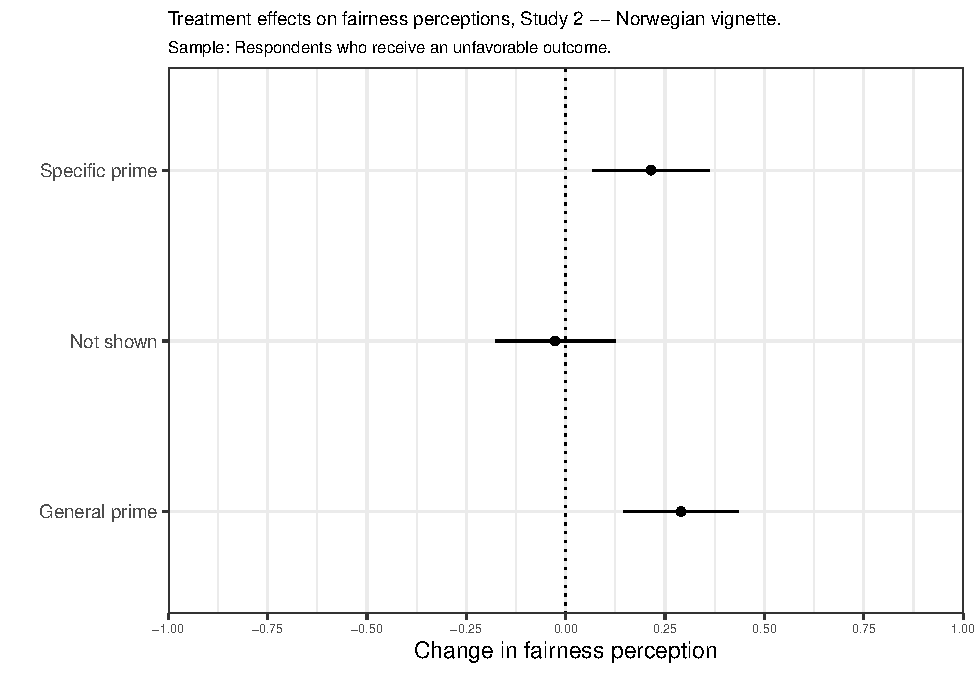
\includegraphics{Goodloser-appendix_files/figure-latex/2055_post_fairness-1.pdf}

Treatment effects among losers on fairness perceptions of decision,
Study 2

Treatment value

Estimate

Std. Error

t-statistic

p value

Intercept

3.77

0.05

70.55

0.00

Generic good loser message

0.29

0.07

4.00

0.00

Not shown

-0.03

0.08

-0.35

0.72

Specific good loser message

0.21

0.07

2.92

0.00

\hypertarget{fairness-moderated-by-issue-importance}{%
\subsection{Fairness moderated by issue
importance}\label{fairness-moderated-by-issue-importance}}

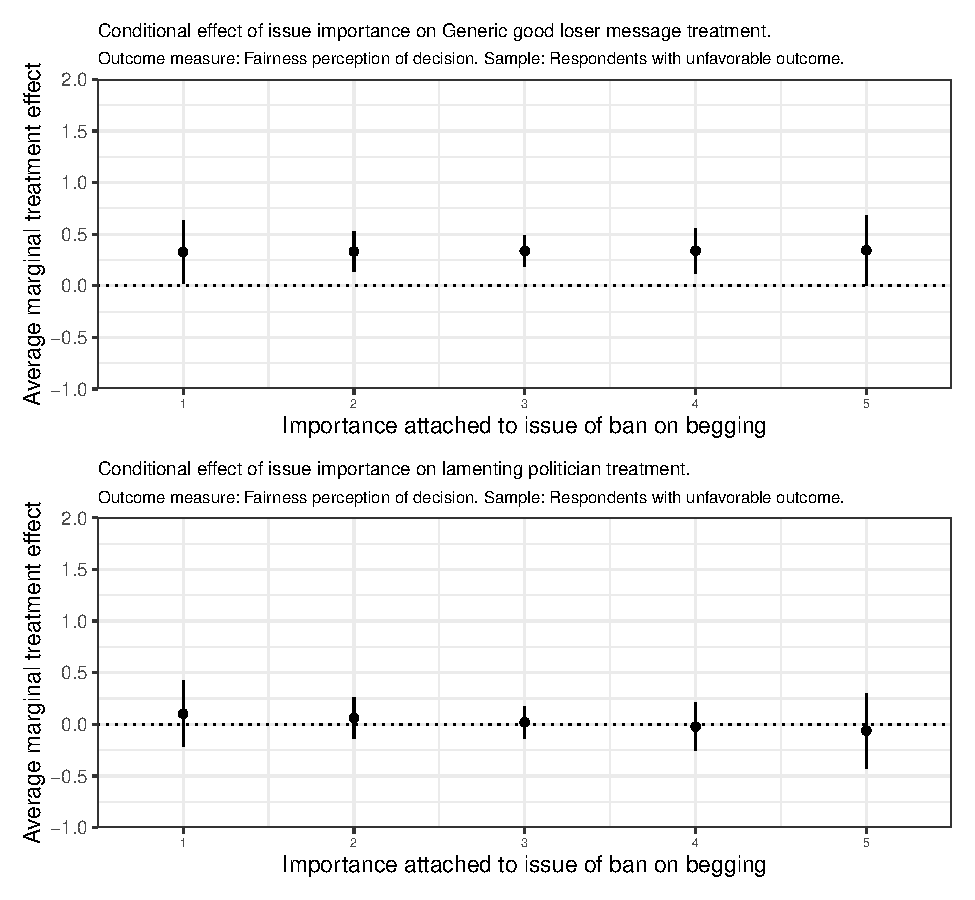
\includegraphics{Goodloser-appendix_files/figure-latex/2050_importance_treatment_fairness-1.pdf}

Moderating effects of issue importance on experimental treatment, Study
2

Factor

Issue importance

AME

SE

z-statistic

p value

Lower

Upper

Generic good loser message

1

0.33

0.15

2.13

0.03

0.03

0.63

Generic good loser message

2

0.33

0.10

3.42

0.00

0.14

0.52

Generic good loser message

3

0.34

0.07

4.56

0.00

0.19

0.48

Generic good loser message

4

0.34

0.11

3.13

0.00

0.13

0.55

Generic good loser message

5

0.34

0.17

2.04

0.04

0.01

0.67

Lamenting politician

1

0.10

0.16

0.65

0.52

-0.21

0.41

Lamenting politician

2

0.06

0.10

0.62

0.53

-0.13

0.25

Lamenting politician

3

0.02

0.08

0.26

0.80

-0.13

0.17

Lamenting politician

4

-0.02

0.12

-0.18

0.86

-0.25

0.21

Lamenting politician

5

-0.06

0.18

-0.34

0.73

-0.42

0.30

{Note: }

Sample: Respondents with unfavorable outcome.

\hypertarget{norm-mod}{%
\subsection{Fairness moderated by good loser norm}\label{norm-mod}}

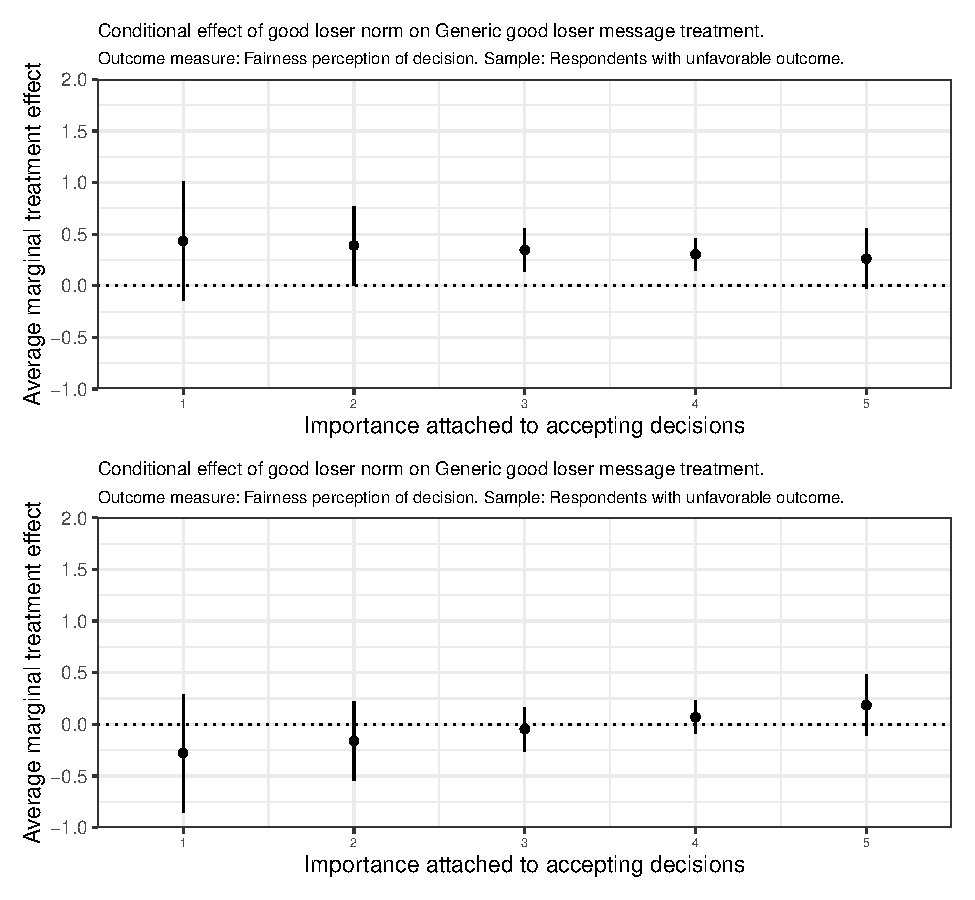
\includegraphics{Goodloser-appendix_files/figure-latex/2050_norm_treatment_fairness-1.pdf}

Moderating effects of norm importance on experimental treatment, Study 2

Factor

Norm importance

AME

SE

z-statistic

p value

Lower

Upper

Generic good loser message

1

0.43

0.29

1.50

0.13

-0.13

1.00

Generic good loser message

2

0.39

0.19

2.03

0.04

0.01

0.76

Generic good loser message

3

0.35

0.11

3.29

0.00

0.14

0.55

Generic good loser message

4

0.30

0.08

3.91

0.00

0.15

0.46

Generic good loser message

5

0.26

0.15

1.79

0.07

-0.03

0.55

Lamenting politician

1

-0.28

0.29

-0.98

0.33

-0.84

0.28

Lamenting politician

2

-0.16

0.19

-0.85

0.39

-0.54

0.21

Lamenting politician

3

-0.05

0.11

-0.43

0.66

-0.26

0.16

Lamenting politician

4

0.07

0.08

0.87

0.39

-0.09

0.23

Lamenting politician

5

0.19

0.15

1.26

0.21

-0.10

0.48

{Note: }

Sample: Respondents with unfavorable outcome.

\hypertarget{willingnes-to-accept}{%
\section{Willingnes to accept}\label{willingnes-to-accept}}

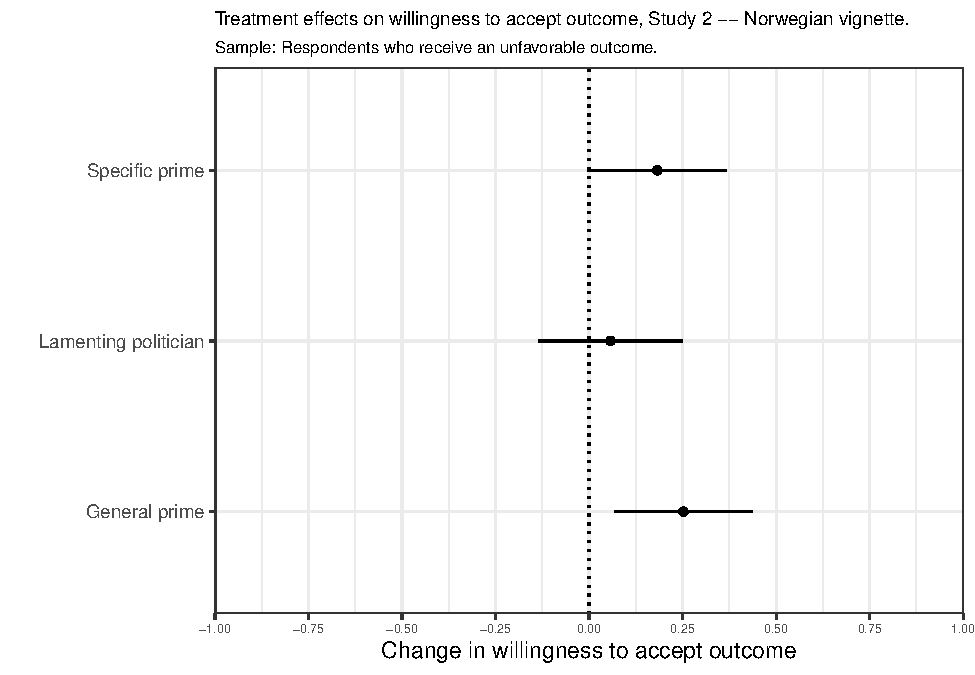
\includegraphics{Goodloser-appendix_files/figure-latex/205_post_accept-1.pdf}

Treatment effects among losers on willingness to accept decision, Study
2

Treatment value

Estimate

Std. Error

t-statistic

p value

Not shown (Intercept)

3.53

0.07

51.98

0.00

Lamenting politician

0.06

0.10

0.60

0.55

Generic good loser message

0.25

0.09

2.74

0.01

Specific good loser message

0.18

0.09

1.96

0.05

\hypertarget{trust-in-politician}{%
\section{Trust in politician}\label{trust-in-politician}}

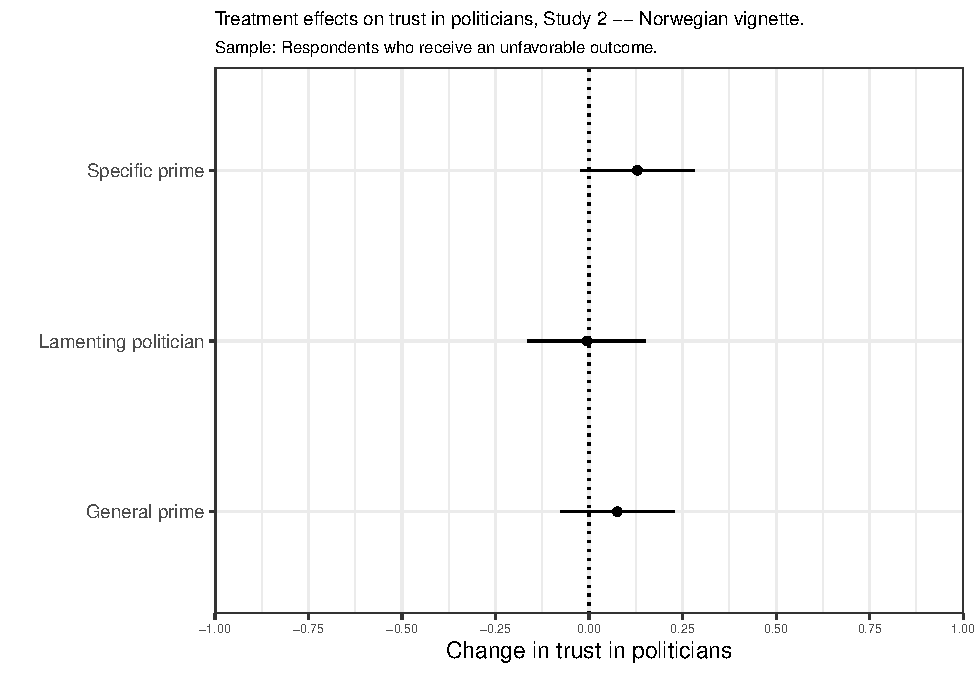
\includegraphics{Goodloser-appendix_files/figure-latex/205_post_trust-1.pdf}

Treatment effects among losers on trust in politician, Study 2

Treatment value

Estimate

Std. Error

t-statistic

p value

Not shown (Intercept)

3.22

0.06

57.66

0.00

Lamenting politician

-0.01

0.08

-0.07

0.94

Generic good loser message

0.08

0.08

1.00

0.32

Specific good loser message

0.13

0.08

1.68

0.09

\hypertarget{reduced-sample}{%
\section{Main effects with reduced sample}\label{reduced-sample}}

\begin{quote}
Main effects with sample that excludes respondents who fail manipulation
check
\end{quote}

\hypertarget{fairness-4}{%
\subsection{Fairness}\label{fairness-4}}

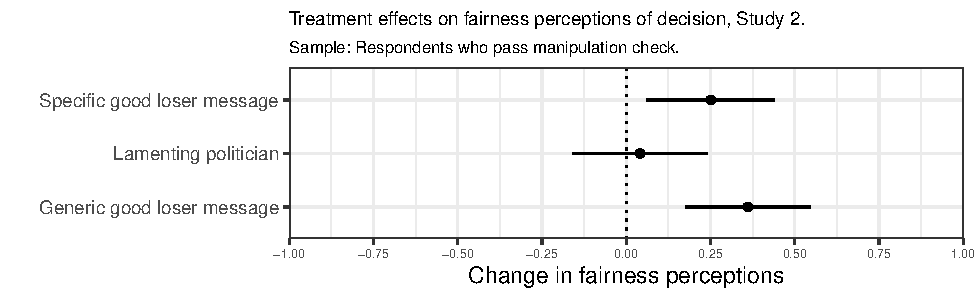
\includegraphics{Goodloser-appendix_files/figure-latex/2045_post_fairness-1.pdf}

Treatment effects on fairness perceptions of decision, Study 2. Sample:
Respondents who pass manipulation check

Treatment value

Estimate

Std. Error

t-statistic

p value

Not shown (Intercept)

3.76

0.07

53.77

0.00

Lamenting politician

0.04

0.10

0.41

0.68

NA

0.36

0.09

3.89

0.00

Specific good loser message

0.25

0.09

2.64

0.01

\hypertarget{willingnes-to-accept-1}{%
\subsection{Willingnes to accept}\label{willingnes-to-accept-1}}

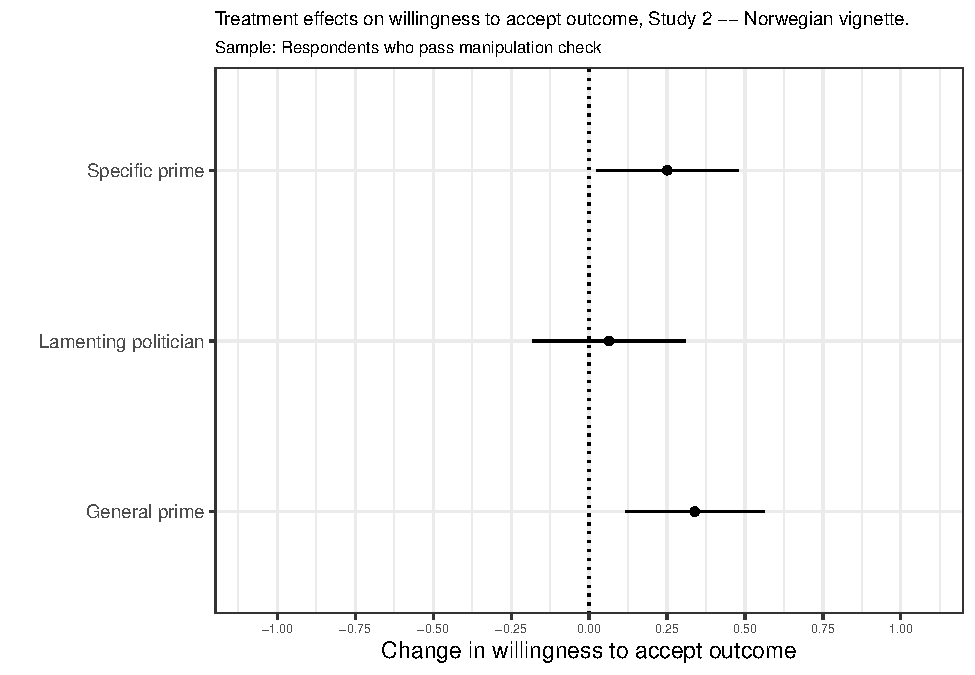
\includegraphics{Goodloser-appendix_files/figure-latex/2045_post_accept-1.pdf}

Treatment effects on willingness to accept decision, Study 2. Sample:
Respondents who pass manipulation check.

Treatment value

Estimate

Std. Error

t-statistic

p value

Not shown (Intercept)

3.45

0.09

37.95

0.00

Lamenting politician

0.06

0.13

0.47

0.64

Generic good loser message

0.34

0.12

2.80

0.01

Specific good loser message

0.25

0.12

2.03

0.04

\hypertarget{trust-in-politician-1}{%
\subsection{Trust in politician}\label{trust-in-politician-1}}

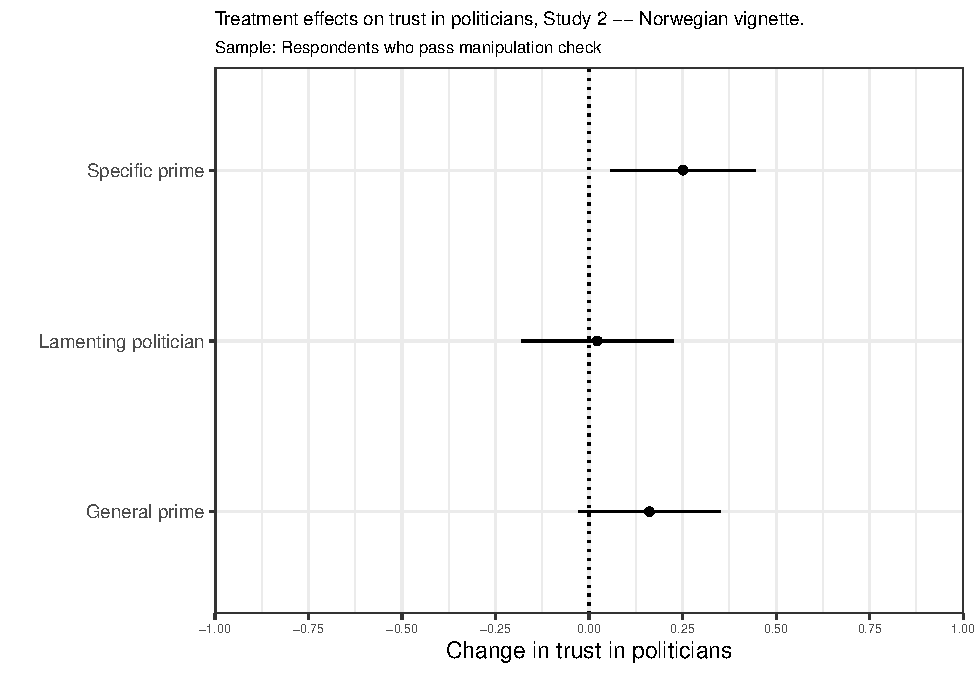
\includegraphics{Goodloser-appendix_files/figure-latex/2045_post_trust-1.pdf}

Treatment effects on trust in politician, Study 2. Sample: Respondents
who pass manipulation check.

Treatment value

Estimate

Std. Error

t-statistic

p value

Not shown (Intercept)

3.17

0.07

42.71

0.00

Lamenting politician

0.02

0.11

0.21

0.83

Generic good loser message

0.16

0.10

1.65

0.10

Specific good loser message

0.25

0.10

2.49

0.01

\hypertarget{part-study-iii}{%
\chapter{(PART) STUDY III}\label{part-study-iii}}

The third study was also run online on a representative sample of adult
Norwegians. We conducted a conjoint experiment with a rating assignment
embedded in the 2018 fall wave of the Norwegian Citizen Panel.

The conjoint design allows us to explore scope conditions of findings.
The advantage of conjoint designs, a method increasingly used in
experimental political science research (Leeper, Hobolt, and Tilley
\protect\hyperlink{ref-leeper2020measuring}{2020}), is the possibility
to include a large number of experimental treatments and estimate their
effects simultaneously (Hainmueller, Hopkins, and Yamamoto
\protect\hyperlink{ref-hainmueller2014causal}{2014}). The stimulus
material for each respondent consists of randomly combined levels of the
given features, resulting in sufficient observations for each feature
while only a small share of the possible combinations is actually shown
to participants. This enables us to include context variables into our
design and to test our relationships of interest across a range of other
factors that could potentially interfere with the treatment. As a result
we gain insights into generalizability and robustness of our findings.
Our conjoint design is presented as a text vignette with rating outcome
measures like in studies 1 and 2. For similar applications in conjoint
designs, see for example Huff and Kertzer
(\protect\hyperlink{ref-huff2018public}{2018}).

\hypertarget{pre-treatment-vignette-post-treatment-1}{%
\chapter{Pre-treatment, vignette,
post-treatment}\label{pre-treatment-vignette-post-treatment-1}}

The statistics are displayed for the respondents of interest in this
study, which is the respondents who end up with observing an unfavorable
decision outcome in the experiment.

\hypertarget{pre-treatment-measures-2}{%
\section{Pre-treatment measures}\label{pre-treatment-measures-2}}

\hypertarget{ban-on-begging---opinion-2}{%
\subsection{Ban on begging - opinion}\label{ban-on-begging---opinion-2}}

What is your opinion on a ban on begging in your municipality?

Value

N

Percent

In favor

836

60

Oppose

553

40

NA

5

0

\hypertarget{ban-on-begging---importance-2}{%
\subsection{Ban on begging -
importance}\label{ban-on-begging---importance-2}}

How important is the issue of begging ban to you?

Value

N

Percent

Not important at all

79

6

Slightly important

251

18

Somewhat important

447

32

Important

517

37

Very important

100

7

The mean score for the pre treatment measure ``How important is the
issue of begging ban to you?'' is 3.55, and the standard deviation is
5.94.

\hypertarget{toll-on-diesel-cars---opinion}{%
\subsection{Toll on diesel cars -
opinion}\label{toll-on-diesel-cars---opinion}}

What is your opinion on an increase in the tolls for diesel cars in your
municipality?

Value

N

Percent

In favor

359

26

Oppose

1026

74

NA

9

1

\hypertarget{toll-on-diesel-cars---importance}{%
\subsection{Toll on diesel cars -
importance}\label{toll-on-diesel-cars---importance}}

How important is the issue of increased tolls for diesel cars to you?

Value

N

Percent

Not important at all

230

16

Slightly important

377

27

Somewhat important

382

27

Important

302

22

Very important

99

7

NA

4

0

The mean score for the pre treatment measure ``How important is the
issue of increased tolls for diesel cars to you?'' is 3.24, and the
standard deviation is 6.96.

\hypertarget{experimental-vignette-2}{%
\section{Experimental vignette}\label{experimental-vignette-2}}

Vignette treatment dimensions and values

Preference

Treatment

Text

Issue

Ban on begging

in the future, begging on the streets will be banned or permitted in the
municipality. This is a controversial decision. Some residents are
strong in favour of a ban (the ``Yes'' side), while other residents are
strongly against a ban (the ``No'' side). Some

Diesel car road toll

in the future, diesel cars will pay increased tolls. This is a
controversial decision. Some residents are strongly in favour of such an
increase (the side), while others are strongly against an increase (the
``No'' side). Some parties propose such an

Outcome

Yes

The Yes side won the vote

No

The No side won the vote

Winning margin

Not shown

.

Small margin

with a slight majority.

Large margin

with a large majority.

Winner's gloating

Not shown

Yes

Following the decision, a politician on the winning side says that it
was a good decision and that common sense prevailed.

Messenger and prime

Not shown

Politician, no prime

The leader of one of the parties that was against the decision says that
they are disappointed and that the decision was wrong.

Politician, specific good loser prime

The leader of one of the parties that was against the decision says that
they are disappointed and that the decision was wrong, but that it was a
fair fight where both sides had the opportunity to argue in favour of
their views.

Politician, generic good loser prime

The leader of one of the parties that was against the decision says that
they are disappointed and that the decision was wrong, but that is what
living in a democracy is all about. Sometimes you win, sometimes you
lose.

Newspaper, no prime

The local newspaper -- which was against the decision -- writes in an
editorial that they are disappointed and that the decision was wrong.

Newspaper, specific good loser prime

The local newspaper -- which was against the decision -- writes in an
editorial that they are disappointed and that the decision was wrong,
but that it was a fair fight where both sides had the opportunity to
argue in favour of their views.

Newspaper, generic good loser prime

The local newspaper -- which was against the decision -- writes in an
editorial that they are disappointed and that the decision was wrong,
but that is what living in a democracy is all about. Sometimes you win,
sometimes you lose.

{Note: }

Experimental vignette (treatments in \{curly brackets\}): Below, we have
described a hypothetical situation. Please read through the situation
carefully and then answer the three questions that follow. Imagine that
your municipality must decide on \{Issue\} The decision will be taken by
the municipal council and follow the usual procedures. The proposal will
initially be debated by the municipal council where all the members will
have the opportunity to express their opinions and arguments regarding
the issue. The debate will be public, and journalists will be in
attendance to report on the debate. In the end, the politicians will
vote on the issue. \{Outcome\} \{{[}Winning margin\} \{Winner gloating\}
\{Messenger and prime\}

\hypertarget{post-treatment-measures-1}{%
\section{Post treatment measures}\label{post-treatment-measures-1}}

Please note that the the respondents were randomly assigned to either a
worded answer scale, or a numbered answer scale. This accounts for the
high share of NA's in the post treatment distribution tables.

\hypertarget{evaluation}{%
\subsection{Evaluation}\label{evaluation}}

What do you think about the way the decision was made?

Value

N

Percent

Not fair at all

104

7

Slightly fair

417

30

Somewhat fair

110

8

Fair

61

4

Very fair

33

2

NA

669

48

What do you think about the way the decision was made?

Value

N

Percent

1 Not fair

252

18

2

190

14

3

135

10

4

42

3

5 Most fair

36

3

NA

739

53

The mean score for the pre treatment measure ``What do you think about
the way the decision was made?'' is 48.71, and the standard deviation is
47.9 for the worded answer scale. For the numbered answer scale, the
mean score is 52.44, and the standard deviation is 47.97

\hypertarget{acceptance-1}{%
\subsection{Acceptance}\label{acceptance-1}}

When you think about the actual outcome of the decision, how willing are
you to accept the decision?

Value

N

Percent

Not willing at all

81

6

Slightly willing

345

25

Somewhat willing

159

11

Willing

106

8

Very willing

36

3

NA

667

48

When you think about the actual outcome of the decision, how willing are
you to accept the decision?

Value

N

Percent

1 Not willing

185

13

2

204

15

3

150

11

4

59

4

5 Most willing

54

4

NA

742

53

The mean score for the pre treatment measure ``When you think about the
actual outcome of the decision, how willing are you to accept the
decision?'' is 48.71, and the standard deviation is 47.86 for the worded
answer scale. For the numbered answer scale, the mean score is 52.61,
and the standard deviation is 47.93

\hypertarget{effects-on-losers-2}{%
\chapter{Effects on losers}\label{effects-on-losers-2}}

Treatment effects on experimental subjects who find the decision outcome
to align unfavorably with their own preferences (N = 1394)

\hypertarget{fairness-perceptions}{%
\section{Fairness perceptions}\label{fairness-perceptions}}

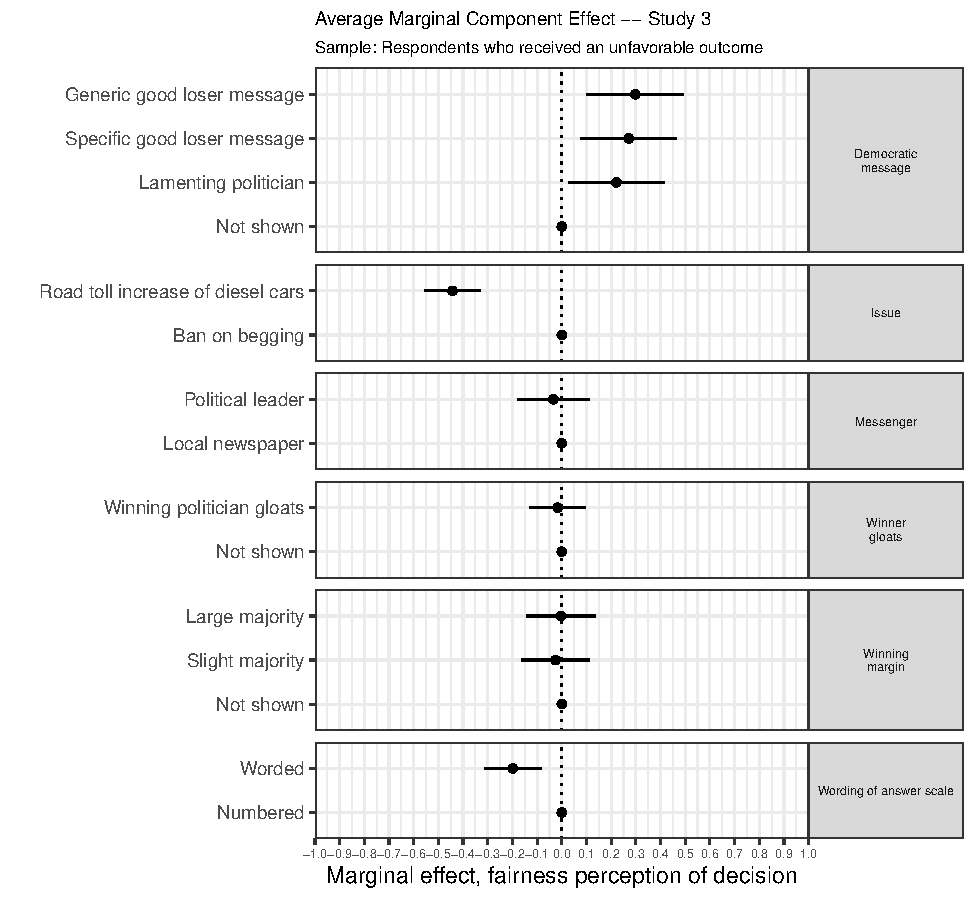
\includegraphics{Goodloser-appendix_files/figure-latex/305_post_fair_loser-1.pdf}

Average Marginal Component Effect -- Study 3

Treatment value

Estimate

Std. Error

t-statistic

p value

Winning margin

Not shown

0.00

0.00

NA

NA

Slight majority

-0.03

0.07

-0.37

0.71

Large majority

0.00

0.07

-0.04

0.97

Winner gloating

Not shown

0.00

0.00

NA

NA

Winning politician gloats

-0.02

0.06

-0.29

0.77

Good loser message

Not shown

0.00

0.00

NA

NA

Lamenting politician

0.22

0.10

2.28

0.02

Specific good loser message

0.27

0.10

2.79

0.01

Generic good loser message

0.30

0.10

3.04

0.00

Messenger

Local newspaper

0.00

0.00

NA

NA

Political leader

-0.03

0.07

-0.46

0.64

Issue

Ban on begging

0.00

0.00

NA

NA

Road toll increase of diesel cars

-0.44

0.06

-7.88

0.00

Wording of answer scale

Numbered

0.00

0.00

NA

NA

Worded

-0.20

0.06

-3.47

0.00

\hypertarget{conditional-amces}{%
\subsection{Conditional AMCEs}\label{conditional-amces}}

Issue importance
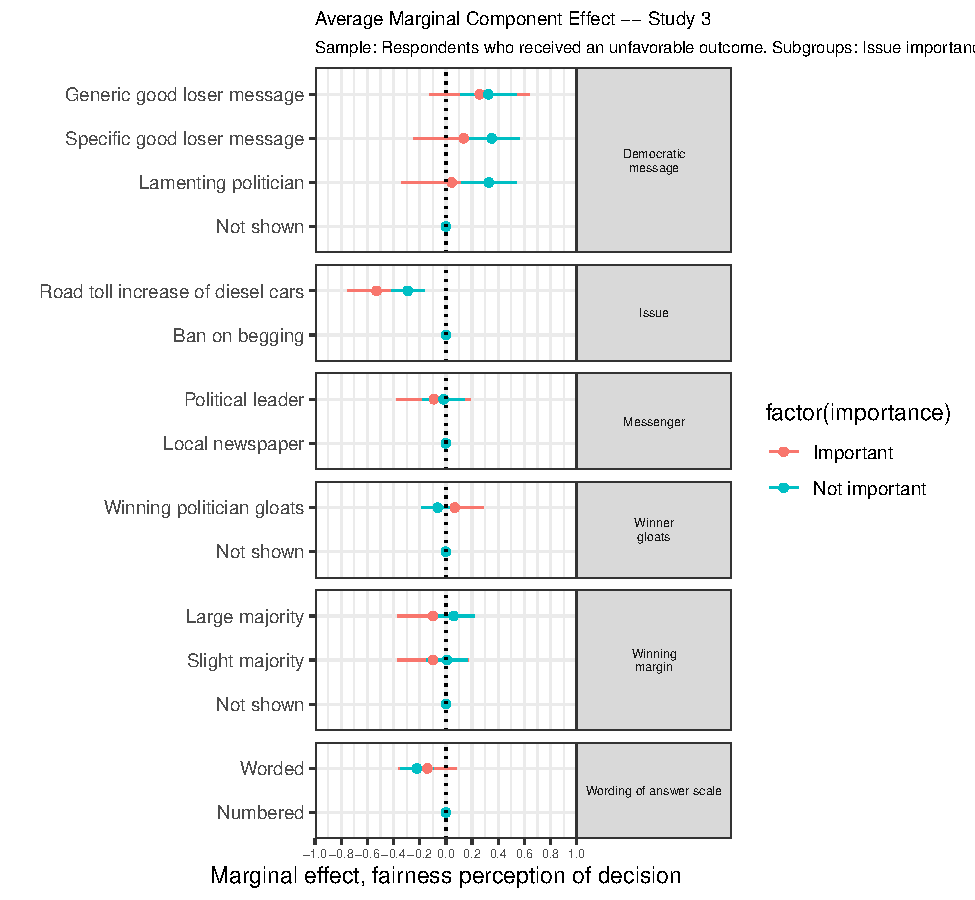
\includegraphics{Goodloser-appendix_files/figure-latex/306_post_fair_losers_intimportance-1.pdf}

Average Marginal Component Effect -- Study 3

Treatment value

Estimate

Std. Error

t-statistic

p value

Issue importance

Winning margin

Not shown

0.00

0.00

NA

NA

Important

Slight majority

-0.10

0.13

-0.73

0.46

Important

Large majority

-0.10

0.13

-0.73

0.47

Important

Not shown

0.00

0.00

NA

NA

Not important

Slight majority

0.01

0.08

0.11

0.91

Not important

Large majority

0.06

0.08

0.75

0.45

Not important

Winner gloating

Not shown

0.00

0.00

NA

NA

Important

Winning politician gloats

0.07

0.11

0.62

0.53

Important

Not shown

0.00

0.00

NA

NA

Not important

Winning politician gloats

-0.06

0.06

-0.98

0.33

Not important

Good loser message

Not shown

0.00

0.00

NA

NA

Important

Lamenting politician

0.04

0.19

0.23

0.82

Important

Specific good loser message

0.14

0.19

0.72

0.47

Important

Generic good loser message

0.26

0.19

1.35

0.18

Important

Not shown

0.00

0.00

NA

NA

Not important

Lamenting politician

0.33

0.11

3.09

0.00

Not important

Specific good loser message

0.35

0.11

3.30

0.00

Not important

Generic good loser message

0.32

0.11

3.04

0.00

Not important

Messenger

Local newspaper

0.00

0.00

NA

NA

Important

Political leader

-0.09

0.14

-0.65

0.51

Important

Local newspaper

0.00

0.00

NA

NA

Not important

Political leader

-0.02

0.08

-0.22

0.83

Not important

Issue

Ban on begging

0.00

0.00

NA

NA

Important

Road toll increase of diesel cars

-0.53

0.11

-4.73

0.00

Important

Ban on begging

0.00

0.00

NA

NA

Not important

Road toll increase of diesel cars

-0.29

0.06

-4.61

0.00

Not important

Wording of answer scale

Numbered

0.00

0.00

NA

NA

Important

Worded

-0.14

0.11

-1.28

0.20

Important

Numbered

0.00

0.00

NA

NA

Not important

Worded

-0.22

0.06

-3.53

0.00

Not important

Issue (ban on begging or road toll)
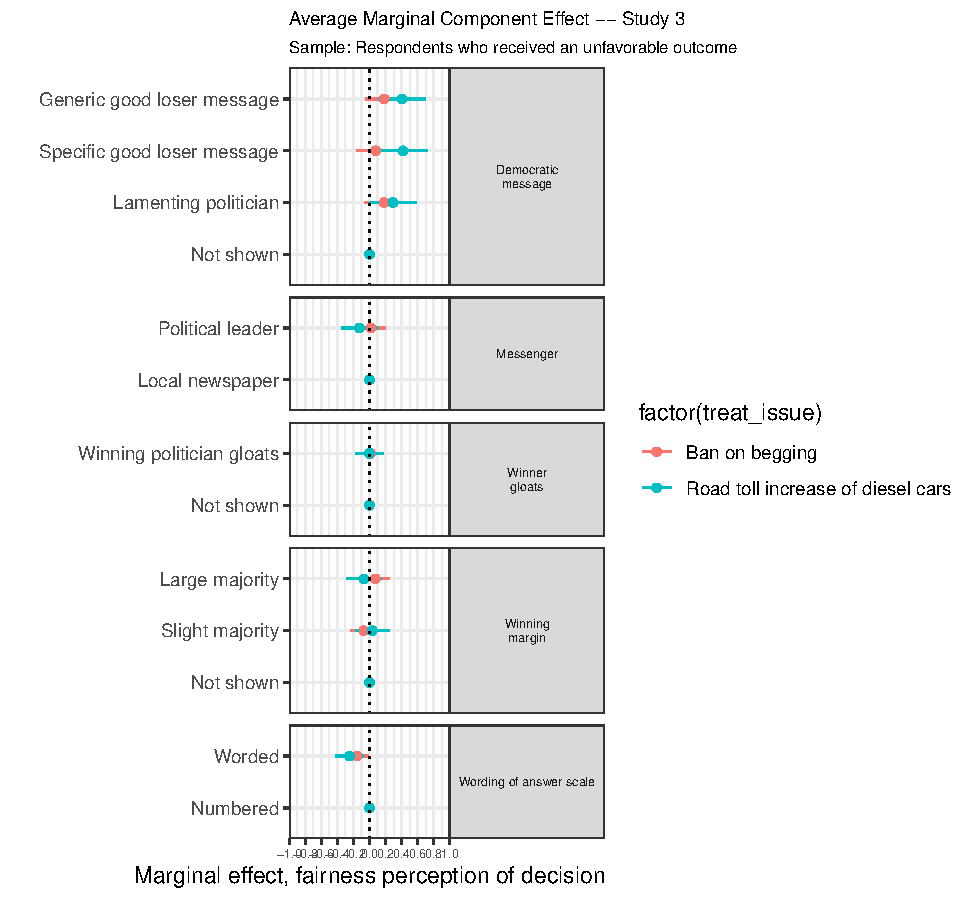
\includegraphics{Goodloser-appendix_files/figure-latex/305_post_fair_loser_issue-1.pdf}

Average Marginal Component Effect -- Study 3

Treatment value

Estimate

Std. Error

t-statistic

p value

Winning margin

Not shown

0.00

0.00

NA

NA

Slight majority

-0.07

0.08

-0.83

0.40

Large majority

0.07

0.09

0.86

0.39

Winner gloating

Not shown

0.00

0.00

NA

NA

Slight majority

0.03

0.11

0.30

0.76

Good loser message

Large majority

-0.07

0.11

-0.63

0.53

Not shown

0.00

0.00

NA

NA

Winning politician gloats

0.01

0.07

0.21

0.83

Not shown

0.00

0.00

NA

NA

Messenger

Winning politician gloats

0.00

0.09

-0.03

0.98

Not shown

0.00

0.00

NA

NA

Issue

Lamenting politician

0.18

0.12

1.50

0.14

Specific good loser message

0.08

0.12

0.65

0.51

Wording of answer scale

Generic good loser message

0.18

0.12

1.53

0.13

Not shown

0.00

0.00

NA

NA

Lamenting politician

0.29

0.15

2.01

0.05

Specific good loser message

0.42

0.15

2.78

0.01

Generic good loser message

0.40

0.15

2.72

0.01

Local newspaper

0.00

0.00

NA

NA

Political leader

0.02

0.09

0.21

0.84

Local newspaper

0.00

0.00

NA

NA

Political leader

-0.13

0.11

-1.10

0.27

Numbered

0.00

0.00

NA

NA

Worded

-0.16

0.07

-2.24

0.03

Numbered

0.00

0.00

NA

NA

Worded

-0.25

0.09

-2.86

0.00

\hypertarget{willingnes-to-accept-2}{%
\section{Willingnes to accept}\label{willingnes-to-accept-2}}

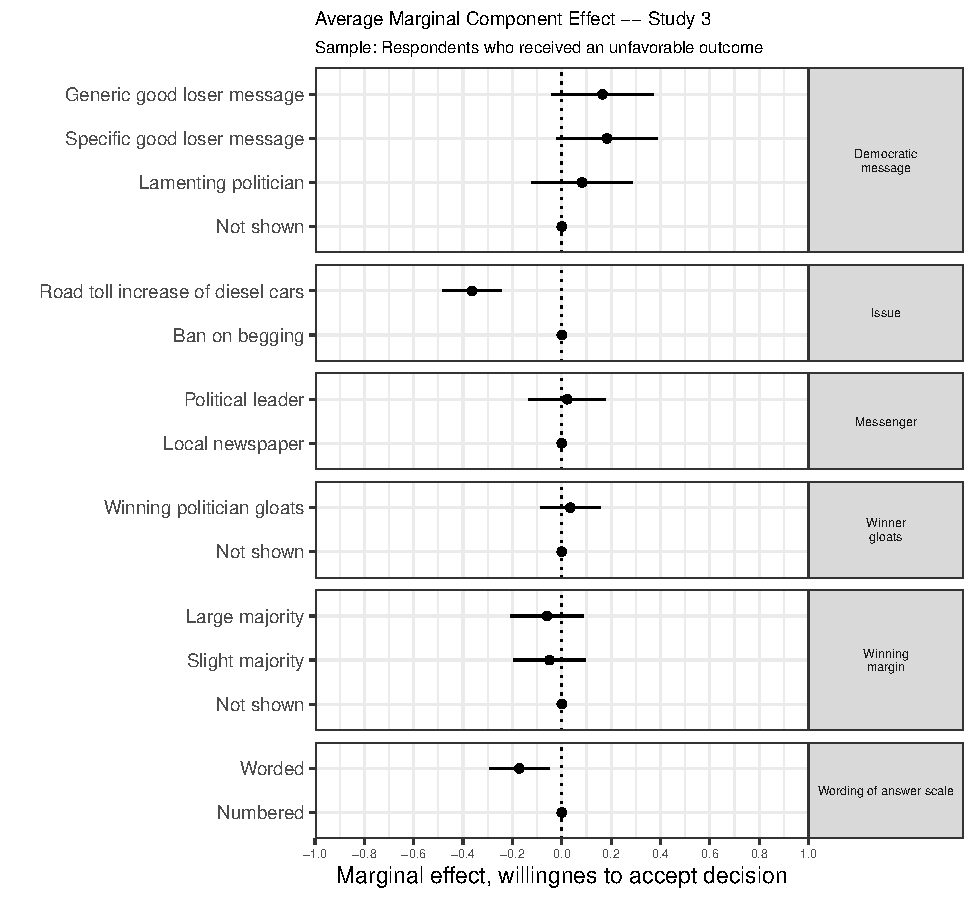
\includegraphics{Goodloser-appendix_files/figure-latex/305_post_accept_loser-1.pdf}

Average Marginal Component Effects -- Study 3

Treatment value

Estimate

Std. Error

t-statistic

p value

Winning margin

Not shown

0.00

0.00

NA

NA

Slight majority

-0.05

0.07

-0.68

0.50

Large majority

-0.06

0.07

-0.80

0.42

Winner gloating

Not shown

0.00

0.00

NA

NA

Winning politician gloats

0.03

0.06

0.57

0.57

Good loser message

Not shown

0.00

0.00

NA

NA

Lamenting politician

0.08

0.10

0.80

0.43

Specific good loser message

0.18

0.10

1.78

0.08

Generic good loser message

0.16

0.10

1.60

0.11

Messenger

Local newspaper

0.00

0.00

NA

NA

Political leader

0.02

0.08

0.28

0.78

Issue

Ban on begging

0.00

0.00

NA

NA

Road toll increase of diesel cars

-0.36

0.06

-6.08

0.00

Wording of answer scale

Numbered

0.00

0.00

NA

NA

Worded

-0.17

0.06

-2.84

0.00

\hypertarget{outcome-favorability-effect-across-the-three-experiments}{%
\chapter{Outcome favorability effect across the three
experiments}\label{outcome-favorability-effect-across-the-three-experiments}}

\begin{quote}
Figure 1 in the manuscript:
\end{quote}

The outcome favorability effect in three experiments

Treatment value

Estimate

Std. Error

t-statistic

p value

Study 1

-0.66

0.08

-8.28

0.00

Study 2

-0.12

0.06

-1.97

0.05

Study 3

-0.30

0.04

-8.15

0.00

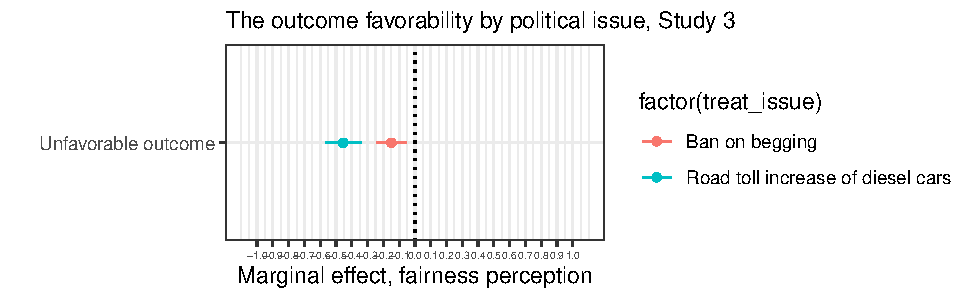
\includegraphics{Goodloser-appendix_files/figure-latex/4044_outfav_issue-1.pdf}

The outcome favorability effect in three experiments

Treatment value

Estimate

Std. Error

t-statistic

p value

Issue

Unfavorable outcome

-0.15

0.05

-3.18

0

Ban on begging

Unfavorable outcome

-0.45

0.06

-7.97

0

Road toll increase of diesel cars

\hypertarget{refs}{}
\leavevmode\hypertarget{ref-hainmueller2014causal}{}%
Hainmueller, Jens, Daniel J Hopkins, and Teppei Yamamoto. 2014. ``Causal
Inference in Conjoint Analysis: Understanding Multidimensional Choices
via Stated Preference Experiments.'' \emph{Political Analysis} 22 (1):
1--30.

\leavevmode\hypertarget{ref-huff2018public}{}%
Huff, Connor, and Joshua D Kertzer. 2018. ``How the Public Defines
Terrorism.'' \emph{American Journal of Political Science} 62 (1):
55--71.

\leavevmode\hypertarget{ref-leeper2020measuring}{}%
Leeper, Thomas J, Sara B Hobolt, and James Tilley. 2020. ``Measuring
Subgroup Preferences in Conjoint Experiments.'' \emph{Political
Analysis} 28 (2): 207--21.

\backmatter
\end{document}
